\documentclass[11pt]{article}
\usepackage[margin=1in]{geometry}
\usepackage[utf8]{inputenc}
\usepackage[T1]{fontenc}
\usepackage{amsmath,amssymb}
\usepackage{booktabs}
\usepackage{enumitem}
\usepackage{tikz}
\usetikzlibrary{arrows.meta,positioning}
\usepackage[hidelinks]{hyperref}

\newcommand{\ARSnode}[1]{%
  \node[circle,draw,minimum size=7mm,inner sep=0pt] (#1) {$#1$};%
}
\newcommand{\ARSnodeat}[2]{%
  \node[circle,draw,minimum size=7mm,inner sep=0pt, #2] (#1) {$#1$};%
}
\tikzset{>={Stealth[length=3mm]}, every loop/.style={looseness=7}}

\title{CPSC 354 — Report}
\author{Ray Hettleman \quad \texttt{rhettleman@chapman.edu}}
\date{\today}

\begin{document}
\maketitle
\tableofcontents

% =========================================================
\section{Assignment 1: MIU System — Can we derive \texttt{MIII} from \texttt{MI}?}

\subsection*{Problem (restated)}
Starting from \texttt{MI}, and using the MIU rules:
\begin{enumerate}[label=\Roman*.]
  \item If a string ends with \texttt{I}, you may append \texttt{U}.
  \item From \texttt{Mx} you may infer \texttt{Mxx}.
  \item Replace any occurrence of \texttt{III} by \texttt{U}.
  \item Delete any occurrence of \texttt{UU}.
\end{enumerate}
Determine whether \texttt{MIII} is derivable. Explain your reasoning.

\subsection*{Solution}
\textbf{Idea.} Track the count of \texttt{I}'s. Rule~I and Rule~IV do not change that count. Rule~II doubles it; Rule~III removes 3 but can only apply if 3 consecutive \texttt{I}'s already exist.

Starting from \texttt{MI} (one \texttt{I}), the only growth is doubling. So after the first step the number of \texttt{I}'s is always even. Removing triples never gives exactly three. So \texttt{MIII} cannot appear.

\subsection*{Conclusion}
It is \textbf{impossible} to derive \texttt{MIII} from \texttt{MI}.  
Reason: the number of \texttt{I}'s is never equal to three under these rules.

% =========================================================
\section{Assignment 2: ARS Pictures \& Properties}

\subsection*{Task (restated)}
For each given abstract reduction system (ARS) $(A,R)$: draw the graph, decide
whether it is terminating, confluent, and whether it has unique normal forms (UNFs).

\subsection*{Instances}

\paragraph{1.\; $A=\varnothing$}
No nodes/edges. \emph{Terminating:} True. \emph{Confluent:} True. \emph{UNFs:} True.

\paragraph{2.\; $A=\{a\},\; R=\varnothing$}
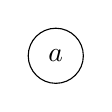
\begin{tikzpicture}
  \ARSnode{a};
\end{tikzpicture}

Normal forms: $a$. Terminating: True. Confluent: True. UNFs: True.

\paragraph{3.\; $A=\{a\},\; R=\{(a,a)\}$}
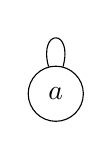
\begin{tikzpicture}
  \ARSnode{a};
  \path (a) edge[loop above] (a);
\end{tikzpicture}

Infinite $a\to a\to\cdots$: Terminating: \textbf{False}. Confluent: \textbf{True}. UNFs: \textbf{False}.

\paragraph{4.\; $A=\{a,b,c\},\; R=\{(a,b),(a,c)\}$}
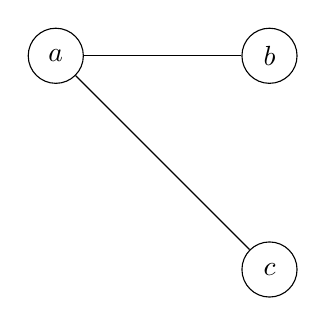
\begin{tikzpicture}[node distance=20mm]
  \ARSnode{a};
  \ARSnodeat{b}{right=of a}
  \ARSnodeat{c}{below=of b}
  \draw (a) edge (b) (a) edge (c);
\end{tikzpicture}

$b,c$ are normal; from $a$ two distinct NFs. Terminating: \textbf{True}. Confluent: \textbf{False}. UNFs: \textbf{False}.

\paragraph{5.\; $A=\{a,b\},\; R=\{(a,a),(a,b)\}$}
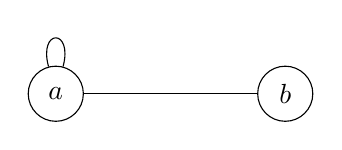
\begin{tikzpicture}[node distance=22mm]
  \ARSnode{a};
  \ARSnodeat{b}{right=of a}
  \draw (a) edge[loop above] (a) (a) edge (b);
\end{tikzpicture}

$b$ is normal; every element has the (unique) NF $b$. Terminating: \textbf{False}. Confluent: \textbf{True}. UNFs: \textbf{True}.

\paragraph{6.\; $A=\{a,b,c\},\; R=\{(a,b),(b,b),(a,c)\}$}
\begin{tikzpicture}[node distance=22mm]
  \ARSnode{a};
  \ARSnodeat{b}{right=of a}
  \ARSnodeat{c}{below=of b}
  \draw (a) edge (b) (a) edge (c) (b) edge[loop above] (b);
\end{tikzpicture}

Non-terminating via $b\to b$; $c$ is normal, $b$ has no NF.
Confluent: \textbf{False}. Terminating: \textbf{False}. UNFs: \textbf{False}.

\paragraph{7.\; $A=\{a,b,c\},\; R=\{(a,b),(b,b),(a,c),(c,c)\}$}
\begin{tikzpicture}[node distance=22mm]
  \ARSnode{a};
  \ARSnodeat{b}{right=of a}
  \ARSnodeat{c}{below=of b}
  \draw (a) edge (b) (a) edge (c) (b) edge[loop above] (b) (c) edge[loop right] (c);
\end{tikzpicture}

Both $b$ and $c$ loop; no NFs reachable from $a$. Terminating: \textbf{False}. Confluent: \textbf{False}. UNFs: \textbf{False}.

\subsection*{Summary Table}
\begin{tabular}{@{}clccc@{}}
\toprule
\# & $(A,R)$ & confluent & terminating & unique normal forms \\
\midrule
1 & $(\varnothing,\varnothing)$ & True & True & True \\
2 & $(\{a\},\varnothing)$ & True & True & True \\
3 & $(\{a\},\{(a,a)\})$ & True & False & False \\
4 & $(\{a,b,c\},\{(a,b),(a,c)\})$ & False & True & False \\
5 & $(\{a,b\},\{(a,a),(a,b)\})$ & True & False & True \\
6 & $(\{a,b,c\},\{(a,b),(b,b),(a,c)\})$ & False & False & False \\
7 & $(\{a,b,c\},\{(a,b),(b,b),(a,c),(c,c)\})$ & False & False & False \\
\bottomrule
\end{tabular}

\subsection*{All 8 combinations}
\begin{tabular}{@{}ccccl@{}}
\toprule
confluent & terminating & unique NFs & example \\
\midrule
True  & True  & True  & e.g.\ ARS 2 (or 1) \\
True  & True  & False & \textit{Impossible} \\
True  & False & True  & ARS 5 \\
True  & False & False & ARS 3 \\
False & True  & True  & \textit{Impossible} \\
False & True  & False & ARS 4 \\
False & False & True  & \textit{Impossible} \\
False & False & False & ARS 6 (or 7) \\
\bottomrule
\end{tabular}

% =========================================================
\section{Assignment 3: Exercises 5 and 5b}

\subsection*{Problem (restated)}
Exercise 5 asks us to analyse a given ARS and check for termination, confluence,
and unique normal forms.  
Exercise 5b asks us to consider a small variation and explain the difference.

\subsection*{Solution to Exercise 5}
For the ARS with $A=\{a,b\}$ and rules $a\to a$, $a\to b$:
\begin{itemize}
  \item There is a loop $a\to a$, so the system is \textbf{not terminating}.
  \item From $a$ we can still reach $b$, and $b$ is normal. Every path from $a$
    eventually has the option to reach $b$, and once at $b$ no rules apply.
  \item Thus the ARS is \textbf{confluent}: all reductions can be joined at $b$.
  \item Normal forms are unique: everything reduces to $b$.
\end{itemize}

\subsection*{Solution to Exercise 5b}
Now suppose we add $c$ with $a\to c$ and $c\to c$:
\begin{itemize}
  \item Again, $a$ can reduce to both $b$ and $c$.
  \item But $c$ loops forever and never reaches $b$.
  \item That means the system is no longer confluent: starting from $a$ you can end
    in either the normal form $b$ or the non-terminating loop on $c$.
  \item Unique normal forms are therefore lost.
\end{itemize}

\subsection*{Conclusion}
Exercise 5 shows a non-terminating but confluent system (everything has the unique NF $b$).  
Exercise 5b shows that adding another looping branch breaks confluence, since from $a$
different outcomes are possible.

% =========================================================
\section{Assignment 4: Termination Exercises}

\subsection*{HW 4.1}
Consider the algorithm:
\begin{verbatim}
while b != 0:
  temp = b
  b = a mod b
  a = temp
return a
\end{verbatim}

This is the Euclidean algorithm for gcd. It terminates whenever $b>0$,
since the measure function $m(a,b)=b$ decreases strictly at each step
and never goes negative.

\subsection*{HW 4.2}
Consider merge sort:
\begin{verbatim}
function merge_sort(arr, left, right):
  if left >= right:
    return
  mid = (left + right) / 2
  merge_sort(arr, left, mid)
  merge_sort(arr, mid+1, right)
  merge(arr, left, mid, right)
\end{verbatim}

We can take as measure function
\[
  \varphi(left,right) = right-left+1.
\]
This is the size of the interval being sorted.
Each recursive call splits the interval into smaller subintervals,
so the measure decreases until it reaches 1, at which point the recursion stops.

% =========================================================
\section{Assignment 5: Lambda Calculus Workout}

\subsection*{Note}
As suggested, I also checked the step sequence in VS Code with Haskell
syntax highlighting (file saved with \texttt{.hs}), which helps match parentheses.

\subsection*{Problem (restated)}
Evaluate
\[
  (\,\lambda f.\,\lambda x.\,f(f(x))\,)\,(\,\lambda f.\,\lambda x.\,f(f(f(x)))\,).
\]

\subsection*{Solution}
\paragraph{Step 1 (parentheses).}
Application associates left; abstractions extend right:
\[
  ((\lambda f.\,\lambda x.\,f(f(x)))\;(\lambda f.\,\lambda x.\,f(f(f(x))))).
\]

\paragraph{Step 2 ($\beta$).}
$(\lambda v.M)\,N \mapsto M[N/v]$ with $v=f$:
\[
  \mapsto\ \lambda x.\, \big((\lambda f.\,\lambda x.\,f(f(f(x))))\big((\lambda f.\,\lambda x.\,f(f(f(x))))\,x\big)\big).
\]

\paragraph{Step 3 ($\alpha$ then $\beta$ inside).}
Rename the inner abstraction’s bound $x$ to $y$ to avoid clashes,
then apply $\beta$:
\[
 (\lambda f.\,\lambda y.\,f(f(f(y))))\,x \mapsto \lambda y.\,x(x(x(y))).
\]

\paragraph{Step 4 ($\beta$ again).}
\[
  \lambda x.\,\big((\lambda f.\,\lambda y.\,f(f(f(y))))(\lambda y.\,x(x(x(y))))\big)
  \mapsto \lambda x.\,\lambda y.\,(\lambda y.\,x(x(x(y))))\,(\lambda y.\,x(x(x(y))))\,(\lambda y.\,x(x(x(y)))).
\]

\paragraph{Step 5 (pattern).}
This denotes nine nested applications of $x$:
\[
  \mapsto\ \lambda x.\,\lambda y.\,x^9(y).
\]

\subsection*{Conclusion}
We practiced $\beta$-reduction, careful substitution, and $\alpha$-conversion;
the composition doubles the triple into a ninefold application.

% =========================================================
\section{Assignment 6: Fixed Point Combinator — Computing \texorpdfstring{$\mathsf{fact}\ 3$}{fact 3}}

\subsection*{Problem (restated)}
Compute the result of
\[
\texttt{let rec fact = \textbackslash n. if n=0 then 1 else n * fact (n-1) in\ 3}
\]
using only the computation rules provided in class for \texttt{fix}, \texttt{let}, and \texttt{let rec}, together with simple
rules for booleans, conditionals, and arithmetic (as suggested on the sheet).

\subsection*{Rules we use (from lecture)}
\begin{align*}
\texttt{fix F} &\;\;\mapsto\;\; \texttt{(F (fix F))} \qquad &\langle\text{rule for \texttt{fix}}\rangle\\
\texttt{let x = e1 in e2} &\;\;\mapsto\;\; \texttt{((\textbackslash x.\ e2)\ e1)} \qquad &\langle\text{def of \texttt{let}}\rangle\\
\texttt{let rec f = e1 in e2} &\;\;\mapsto\;\; \texttt{let f = (fix (\textbackslash f.\ e1)) in e2} \qquad &\langle\text{def of \texttt{let rec}}\rangle
\end{align*}
For the arithmetic/boolean side (as recommended):\\
\texttt{0=0 $\mapsto$ True}, \quad \texttt{1=0 $\mapsto$ False}, \quad
\texttt{if True then A else B $\mapsto$ A}, \quad
\texttt{if False then A else B $\mapsto$ B}, \\
\texttt{2*1 $\mapsto$ 2}, \quad \texttt{3*2 $\mapsto$ 6}, \quad \texttt{3-1 $\mapsto$ 2}, \quad \texttt{2-1 $\mapsto$ 1}, etc.

\subsection*{Abbreviation}
For readability let
\[
\texttt{F} \;\; \equiv \;\; \texttt{\textbackslash fact.\ \textbackslash n.\ if n=0 then 1 else n * fact (n-1)}.
\]

\subsection*{Computation}
We now reduce, labeling every step with the rule name (matching the sheet).

\medskip
\noindent
\texttt{let rec fact = \textbackslash n. if n=0 then 1 else n * fact (n-1) in 3}\\
\(\to\) \texttt{let fact = (fix (\textbackslash fact.\ \textbackslash n.\ if n=0 then 1 else n * fact (n-1))) in 3}
\hfill \(\langle\)def of \texttt{let rec}\(\rangle\)

\medskip
\noindent
\(\to\) \texttt{((\textbackslash fact.\ 3)\ (fix (\textbackslash fact.\ \textbackslash n.\ if n=0 then 1 else n * fact (n-1))))}
\hfill \(\langle\)def of \texttt{let}\(\rangle\)

\medskip
\noindent
\(\to\) \texttt{3} \quad with an environment binding
\texttt{fact := (fix (\textbackslash fact.\ \textbackslash n.\ if n=0 then 1 else n * fact (n-1)))}.
\hfill \(\langle\beta\rangle\)

\medskip

But to \emph{evaluate} \texttt{fact 3} we unfold \texttt{fix} as needed:

\begin{align*}
\texttt{fact} &= \texttt{fix (\textbackslash fact.\ \textbackslash n.\ if n=0 then 1 else n * fact (n-1))}\\
&= \texttt{fix F} \\
&\mapsto \texttt{(F (fix F))} && \langle\text{rule for \texttt{fix}}\rangle\\
&= \texttt{(\textbackslash fact.\ \textbackslash n.\ if n=0 then 1 else n * fact (n-1)) (fix F)}\\
&\mapsto \texttt{\textbackslash n.\ if n=0 then 1 else n * (fix F)\ (n-1)} && \langle\beta\rangle
\end{align*}

Now apply this to \texttt{3}:

\begin{align*}
\texttt{fact 3}
&\mapsto \texttt{if 3=0 then 1 else 3 * (fix F)\ (3-1)} && \langle\beta\rangle\\
&\mapsto \texttt{if False then 1 else 3 * (fix F)\ 2} && \langle 3=0 \mapsto \text{False}\rangle\\
&\mapsto \texttt{3 * (fix F)\ 2} && \langle \text{if False}\rangle
\end{align*}

Unfold \texttt{fix} again to compute \texttt{(fix F)\ 2}:

\begin{align*}
\texttt{(fix F)}
&\mapsto \texttt{(F (fix F))} && \langle\text{rule for \texttt{fix}}\rangle\\
&\mapsto \texttt{\textbackslash n.\ if n=0 then 1 else n * (fix F)\ (n-1)} && \langle\beta\rangle
\end{align*}

So
\begin{align*}
\texttt{(fix F)\ 2}
&\mapsto \texttt{if 2=0 then 1 else 2 * (fix F)\ (2-1)} && \langle\beta\rangle\\
&\mapsto \texttt{2 * (fix F)\ 1} && \langle 2=0 \mapsto \text{False},\ \text{if False}\rangle
\end{align*}

Again unfold for the \texttt{1} case:
\begin{align*}
\texttt{(fix F)\ 1}
&\mapsto \texttt{if 1=0 then 1 else 1 * (fix F)\ (1-1)} && \langle\beta\rangle\\
&\mapsto \texttt{if False then 1 else 1 * (fix F)\ 0} && \langle 1=0 \mapsto \text{False}\rangle\\
&\mapsto \texttt{1 * (fix F)\ 0} && \langle \text{if False}\rangle
\end{align*}

Base case:
\begin{align*}
\texttt{(fix F)\ 0}
&\mapsto \texttt{if 0=0 then 1 else 0 * (fix F)\ (-1)} && \langle\beta\rangle\\
&\mapsto \texttt{1} && \langle 0=0 \mapsto \text{True},\ \text{if True}\rangle
\end{align*}

So back-substituting:
\[
\texttt{(fix F)\ 1} \mapsto \texttt{1 * 1} \mapsto \texttt{1}.
\]

Then
\[
\texttt{(fix F)\ 2} \mapsto \texttt{2 * 1} \mapsto \texttt{2}.
\]

Finally
\[
\texttt{fact 3} \mapsto \texttt{3 * 2} \mapsto \texttt{6}.
\]

\subsection*{Conclusion}
Following only the lecture’s computation rules and the suggested simple arithmetic/boolean reductions, the program
\[
\texttt{let rec fact = \textbackslash n. if n=0 then 1 else n * fact (n-1) in 3}
\]
reduces to \textbf{\texttt{6}}. The trace shows the pattern of unfolding \texttt{fix} exactly when needed and using \(\beta\)-reductions together with the conditional rules. (I also mirrored the lecture style of naming each rule beside the step, and verified parentheses in VS Code with Haskell highlighting.)

\end{document}
